\section{Использование TCP для передачи данных}


В качестве точки отсчета в настоящей работе выступает метод межпроцессного взаимодействия на основе TCP, используемый посредством сокетов 
%\textbf{TBD: ссылка на определение}
\ref{chapter31:PureTCP}.

Показатели потока исходящих заявок из симулятора в данном эксперименте: $\Delta \in$ \textit{10 $\pm$ 4 мс}, $\delta \in$ \textit{50 $\pm$ 26 мкс}.

\begin{figure}[!h]
\caption{Гистограмма временной задержки на передачу данных между процессами при использовании TCP}
\label{chapter41:FigPureTCP}
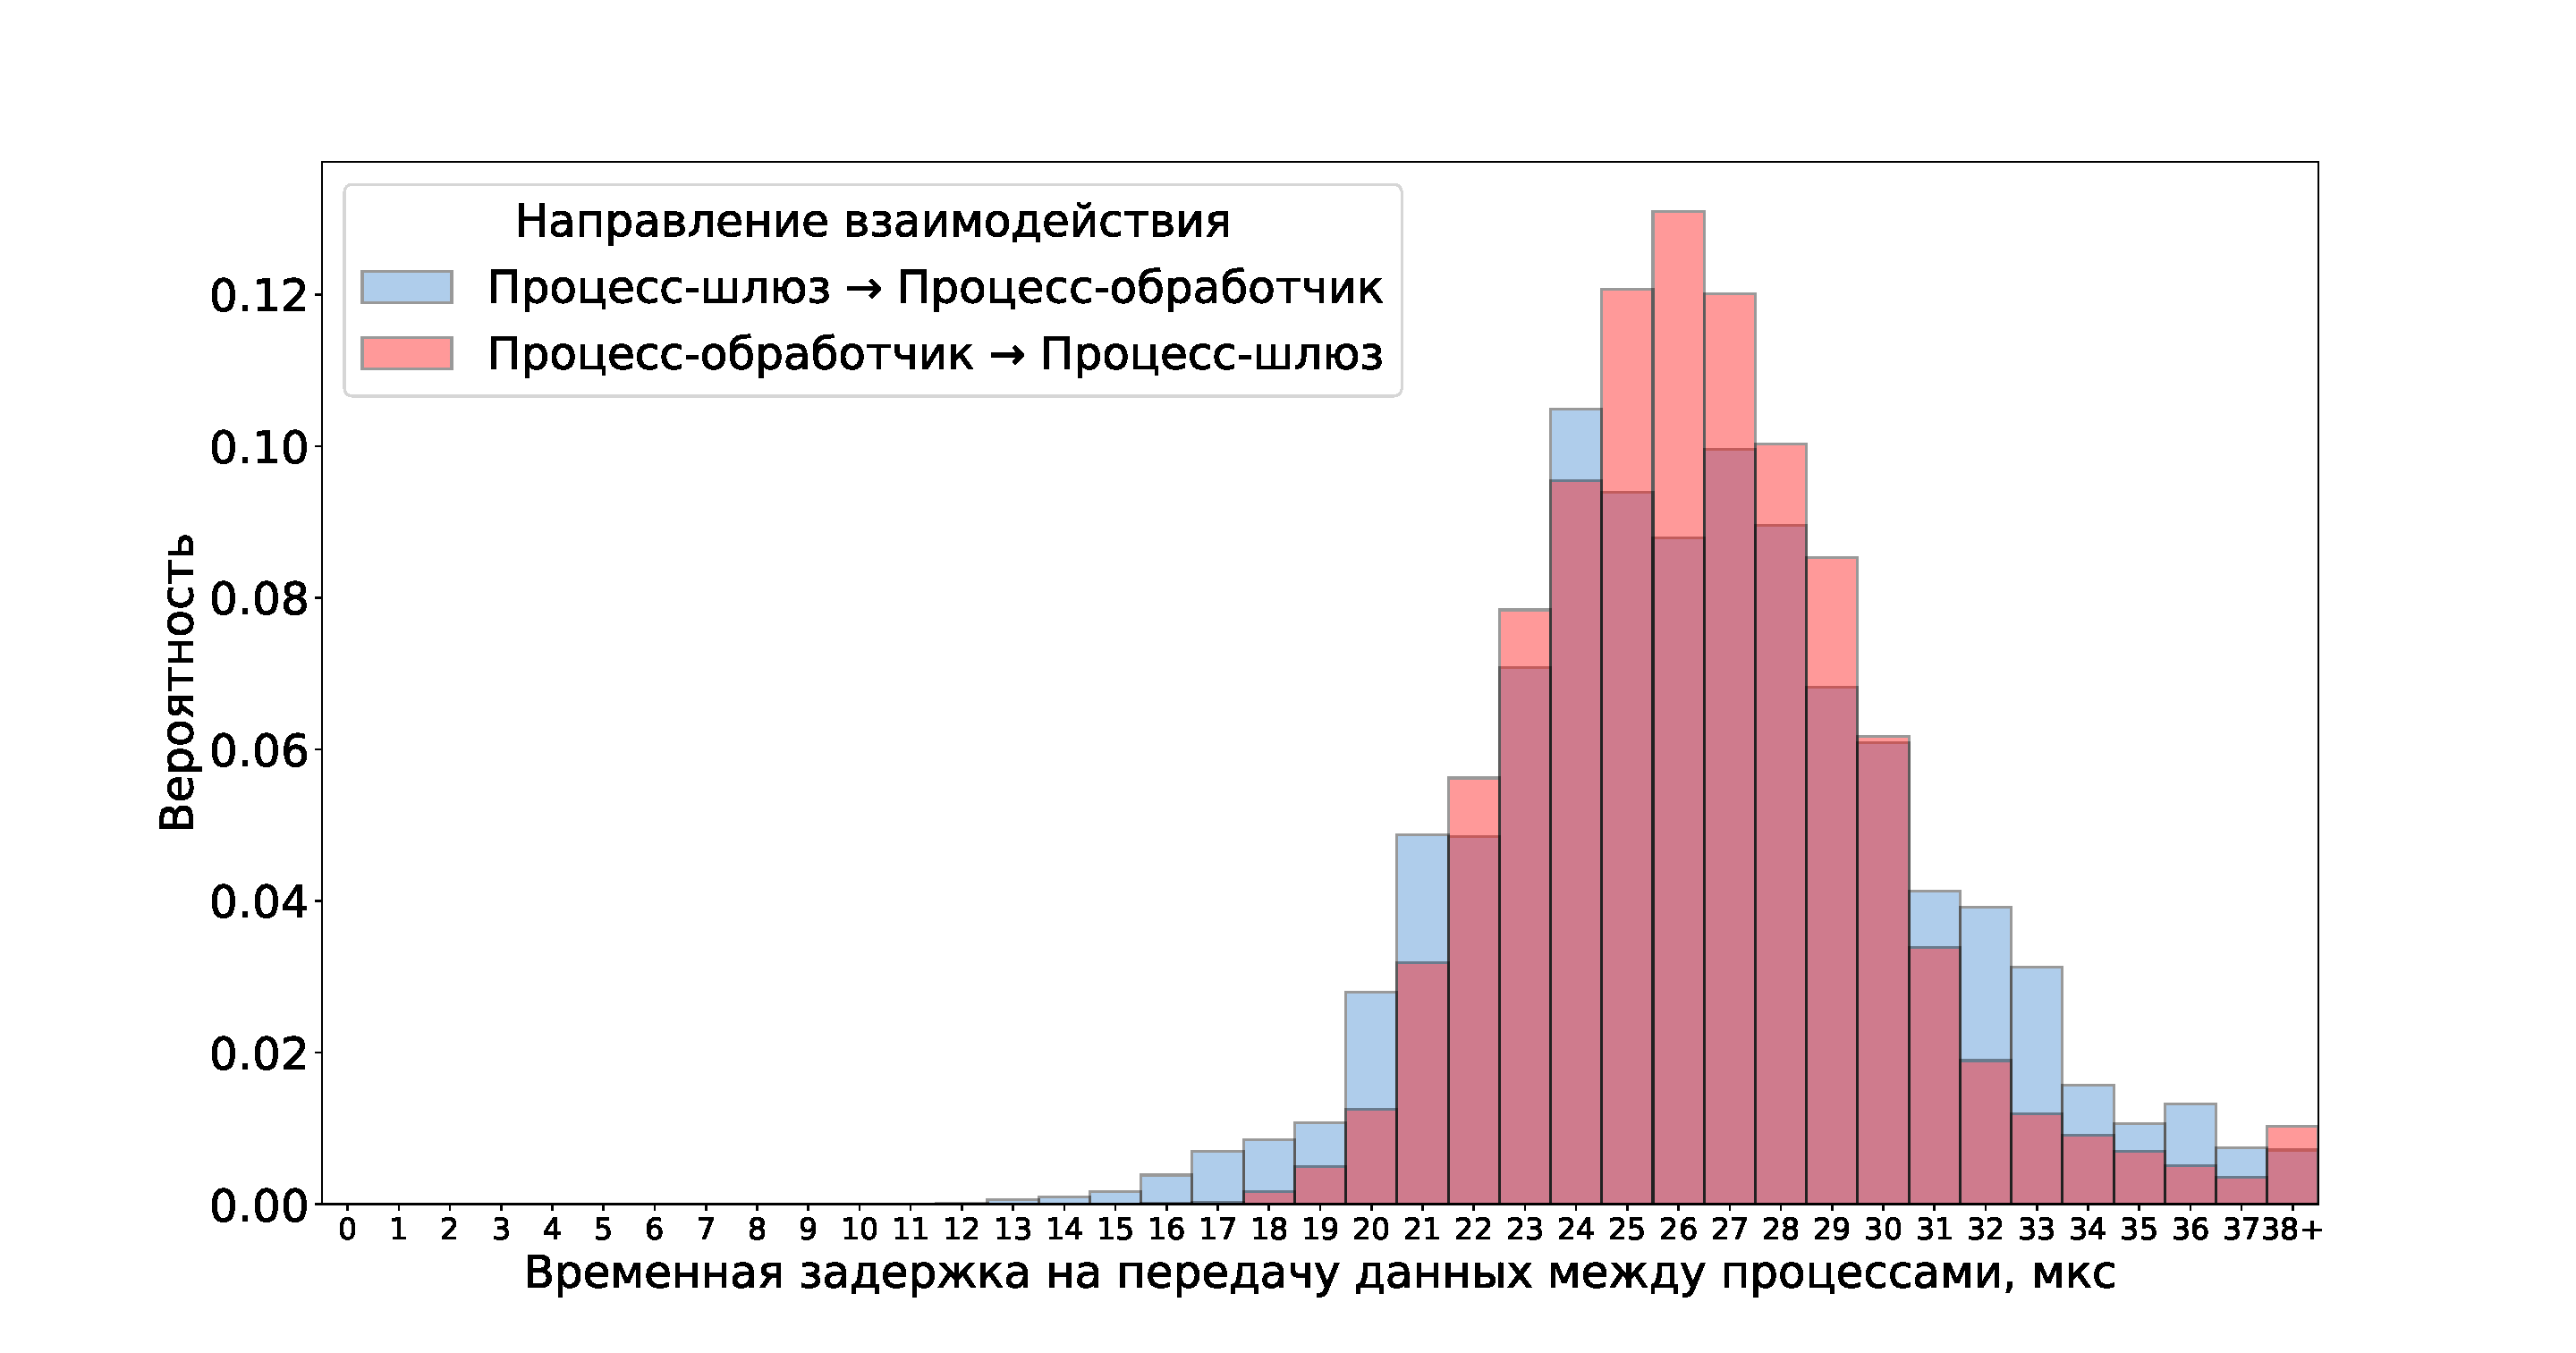
\includegraphics[width=\textwidth]{../../graphics/hist/PureTCP}
\end{figure}

Гистограмма временной задержки на передачу данных для данного метода приведена на Рисунке \ref{chapter41:FigPureTCP}. В Таблице \ref{chapter41:TablePureTCP} приведены основные временные характеристики данного метода.

\begin{table}[!h]
\caption{Основные показатели временной задержки на передачу данных для метода на основе TCP}\label{chapter41:TablePureTCP}
\centering
\begin{tabular}{|l|c|c|}
\hline
\begin{tabular}[c]{@{}l@{}}Направление\\ взаимодействия/\\ Показатель\end{tabular} & \multicolumn{1}{l|}{\begin{tabular}[c]{@{}l@{}}Процесс-шлюз $\rightarrow$\\ Процесс-обработчик\end{tabular}} & \multicolumn{1}{l|}{\begin{tabular}[c]{@{}l@{}}Процесс-обработчик $\rightarrow$\\ Процесс-шлюз\end{tabular}} \\ \hline
min(t), мкс & 9 & 13 \\ \hline
M(t), мкс & 27.5 $\pm$ 8.5 & 28 $\pm$ 7 \\ \hline
max(t), мс & 2.1 & 9.2 \\ \hline
\begin{tabular}[c]{@{}l@{}}$\Delta$, мс\end{tabular} & 10 $\pm$ 4 & 10 $\pm$ 4 \\ \hline
\begin{tabular}[c]{@{}l@{}}$\delta$, мкс\end{tabular} & 50 $\pm$ 26 & 87 $\pm$ 32 \\ \hline
\end{tabular}
\end{table}

Временная задержка на передачу данных в обоих направлениях имеет схожие значения. Это объясняется тем, что накладные расходы на использование TCP через механизм сокетов имеют подавляющее значение над прочими факторами, влияющими на межпроцессное взаимодействие.

\section{Использование разделяемой памяти для передачи данных}

\subsection{Использование TCP для оповещения о появлении данных}

Показатели потока исходящих заявок из симулятора в данном эксперименте: $\Delta \in$ \textit{10 $\pm$ 4 мс}, $\delta \in$ \textit{50 $\pm$ 27 мкс}.

В данном подразделе приведены данные об экспериментах с методом межпроцессного взаимодействия, описанным в Разделе \ref{chapter31:SignalTCP}.

\begin{figure}[!h]
\caption{Гистограмма временной задержки на передачу данных между процессами при использовании разделяемой памяти для передачи данных и TCP для оповещения о появлении данных в ней}
\label{chapter41:FigSignalTCP}
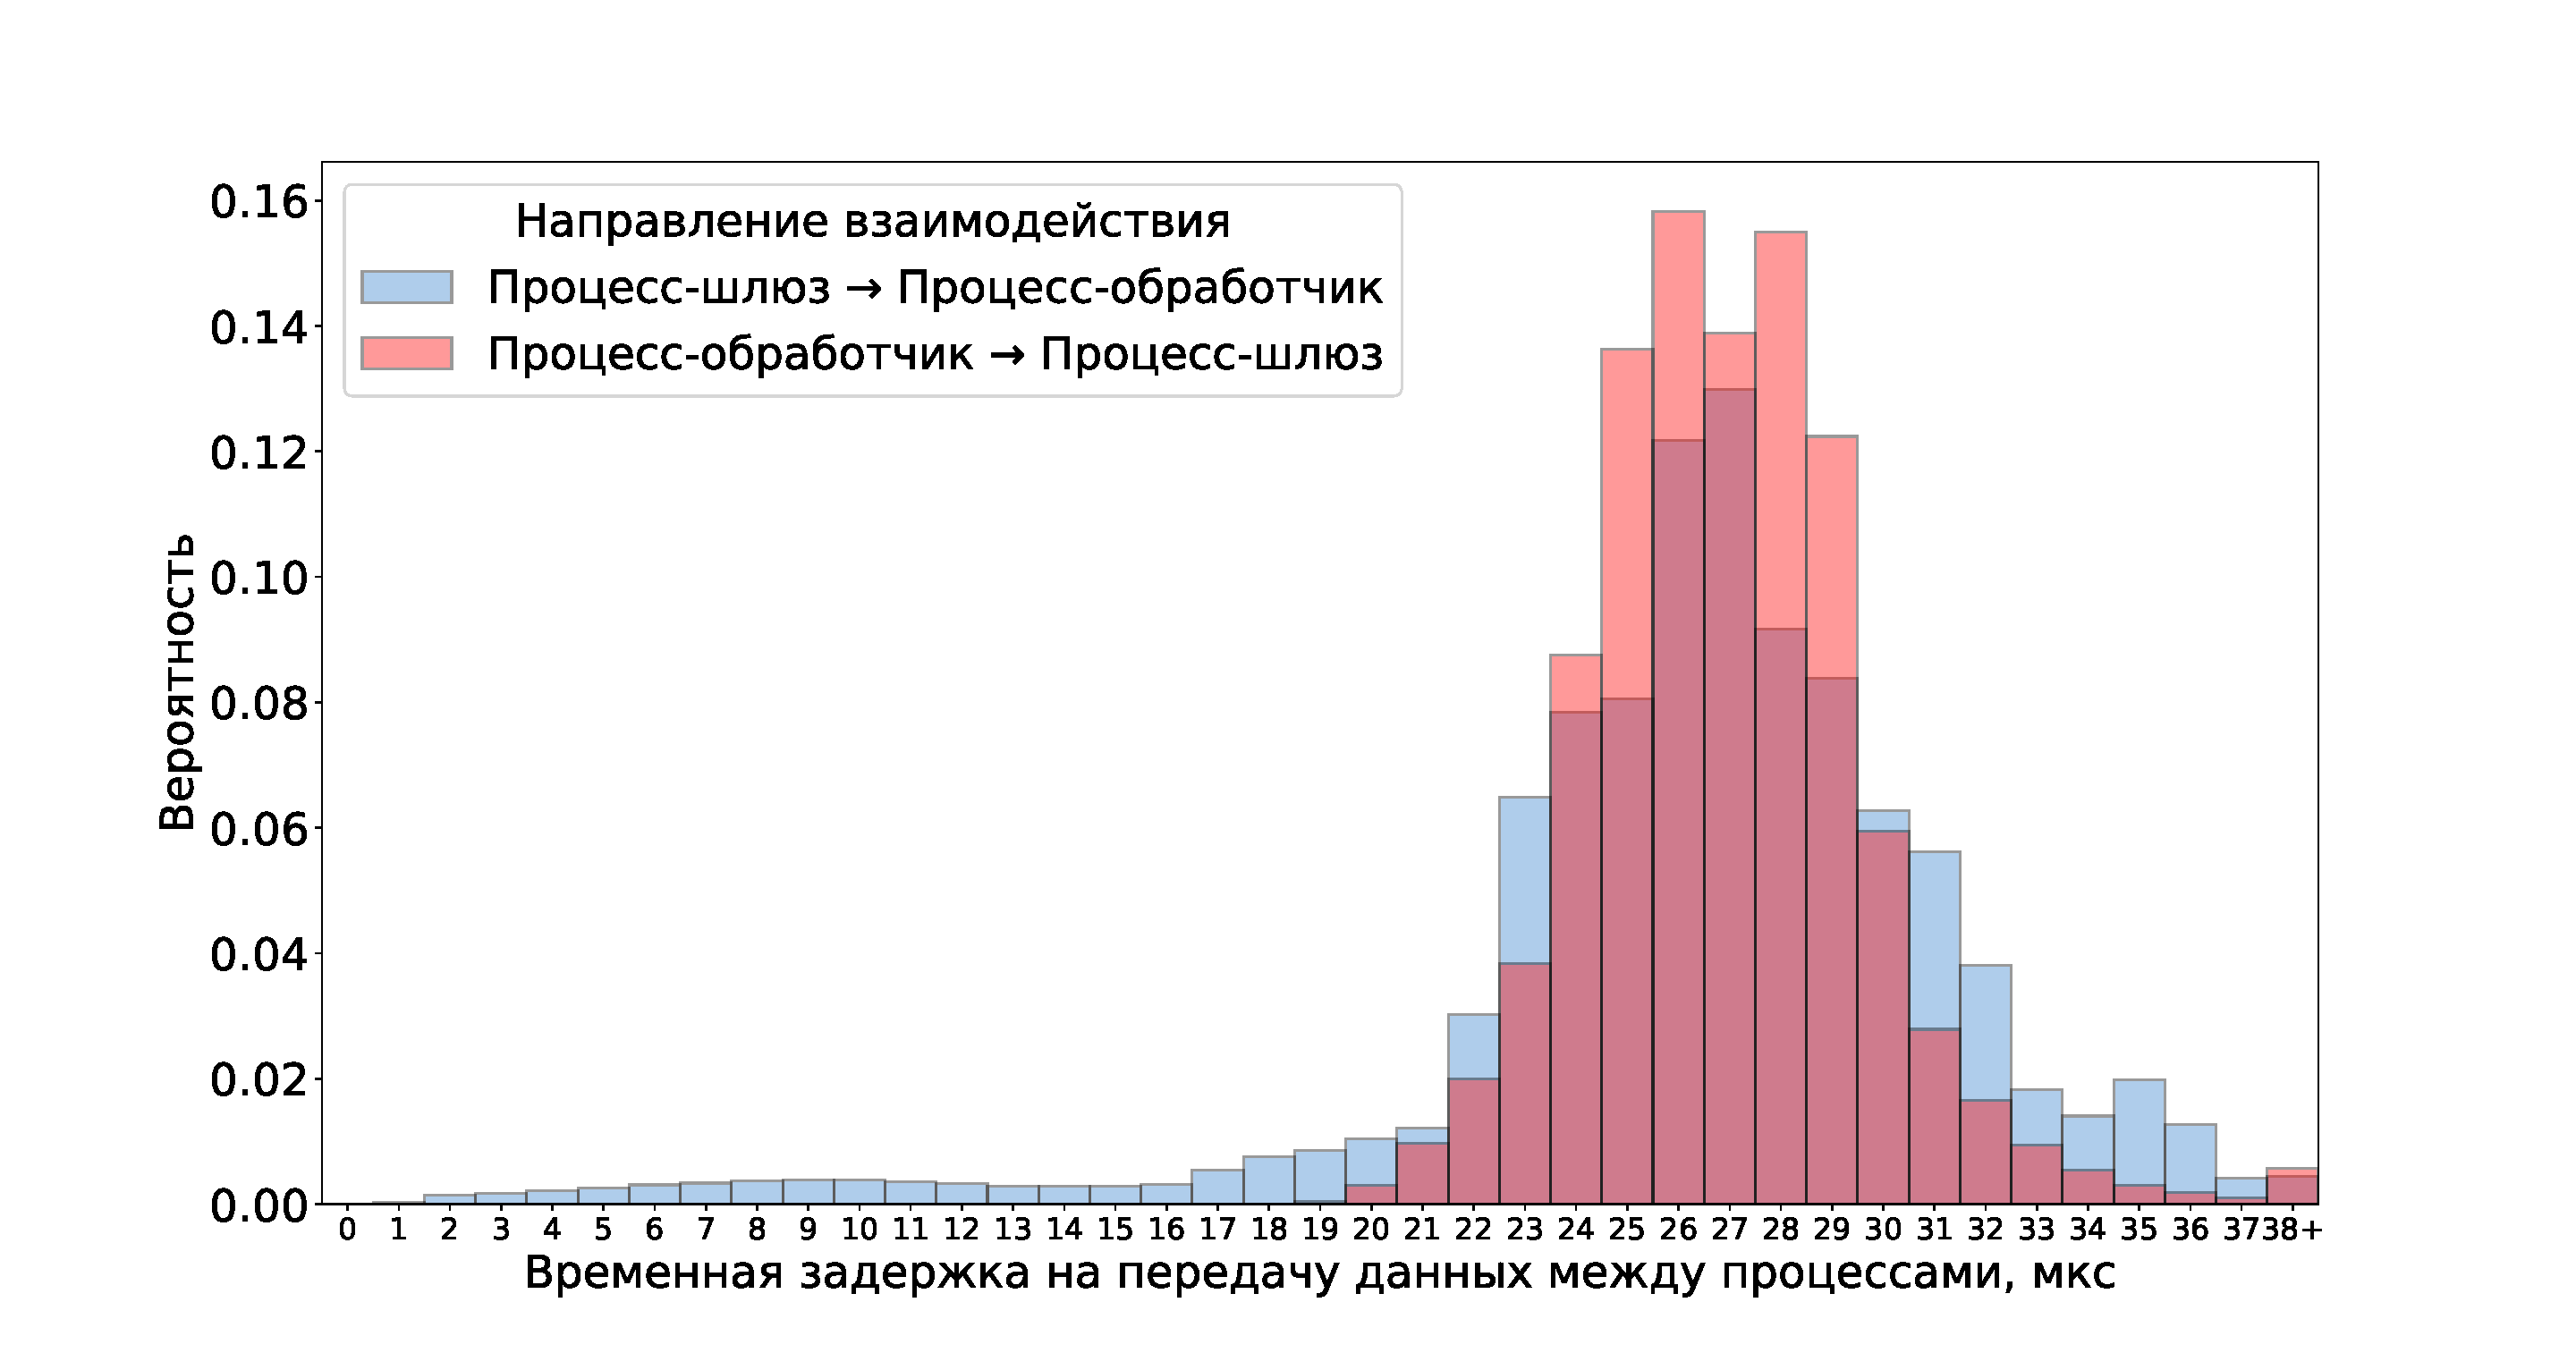
\includegraphics[width=\textwidth]{../../graphics/hist/SignalTCP}
\end{figure}

\begin{table}[!h]
\caption{Основные показатели временной задержки на передачу данных для метода, использующего разделяемую памяти для передачи данных и TCP для оповещения о появлении данных в ней}\label{chapter41:TableSignalTCP}
\centering
\begin{tabular}{|l|c|c|}
\hline
\begin{tabular}[c]{@{}l@{}}Направление\\ взаимодействия/\\ Показатель\end{tabular} & \multicolumn{1}{l|}{\begin{tabular}[c]{@{}l@{}}Процесс-шлюз $\rightarrow$\\ Процесс-обработчик\end{tabular}} & \multicolumn{1}{l|}{\begin{tabular}[c]{@{}l@{}}Процесс-обработчик $\rightarrow$\\ Процесс-шлюз\end{tabular}} \\ \hline
min(t), мкс & 1 & 3 \\ \hline
M(t), мкс & 22.5 $\pm$ 12.5 & 27.5 $\pm$ 5.5 \\ \hline
max(t), мс & 3 & 9.8 \\ \hline
\begin{tabular}[c]{@{}l@{}}$\Delta$, мс\end{tabular} & 10 $\pm$ 4 & 10 $\pm$ 4 \\ \hline
\begin{tabular}[c]{@{}l@{}}$\delta$, мкс\end{tabular} & 50 $\pm$ 27 & 87 $\pm$ 32 \\ \hline
\end{tabular}
\end{table}

В Таблице \ref{chapter41:TableSignalTCP} приведены основные временные характеристики данного метода. На Рисунке \ref{chapter41:FigSignalTCP} приведена гистограмма временной задержки на передачу данных для данного метода.

Как описано выше, значительная часть обслуживания заявки процессом-обработчиком происходит непосредственно в транспортном потоке. Из-за этого к моменту конца обработки текущей заявки очередная заявка уже может находиться в очереди в разделяемой памяти, что позволяет использовать оптимизацию, описанную в Разделе \ref{chapter31:SharedMemoryOptimization}. А именно принять и начать обслуживание очередной заявки, не используя дорогостоящий механизм оповещения, если заявка уже находится в очереди в разделяемой памяти. 

Прием заявки процессом-шлюзом не связан с обслуживанием заявки, поэтому к моменту, когда процесс-шлюз заканчивает прием и диспетчеризацию заявки, очередь входящих заявок в данном эксперименте пуста и поток-шлюз переходит к пассивному ожиданию новых заявок. Таким образом, приему и обслуживанию большинства заявок сопутствует пассивное ожидание сигнала по TCP, что негативно сказывается на временной задержке на передачу данных.

\subsection{Использование мультиплексора в разделяемой памяти для оповещения о появлении данных}

В данном подразделе приведены данные об экспериментах с семейством методов межпроцессного взаимодействия, описанными в Разделе \ref{chapter31:Mux}.

\subsubsection{Методы с пассивным ожиданием оповещений}

В методах с пассивным ожиданием оповещений поток мультиплексора событий использует примитив \textit{futex} 
% \textbf{TBD:Может, сослаться на определение futex?}
для ожидания новых сигналов (см. Разделы \ref{chapter31:BlockingHSHA} и \ref{chapter31:BlockingLF}). Поток процесса-читателя, опрашивающий мультиплексор в разделяемой памяти, находится в состоянии сна и пробуждается процессом-писателем при необходимости.

\paragraph{Диспетчеризация и обработка соединений по модели "Полусинхронный/Полуреактивный"}

Показатели потока исходящих заявок из симулятора в данном эксперименте: $\Delta \in$ \textit{10 $\pm$ 4 мс}, $\delta \in$ \textit{51 $\pm$ 28 мкс}.

В данном подразделе приведены данные об экспериментах с методом межпроцессного взаимодействия, описанным в Разделе \ref{chapter31:BlockingHSHA}.

\begin{figure}[!h]
\caption{Гистограмма временной задержки на передачу данных между процессами для метода, использующего разделяемую память для передачи данных, пассивное ожидание событий на мультиплексоре событий в разделяемой памяти и метод ''Полусинхронный/Полуреактивный`` при обслуживании заявок}
\label{chapter41:FigBlockingHSHA}
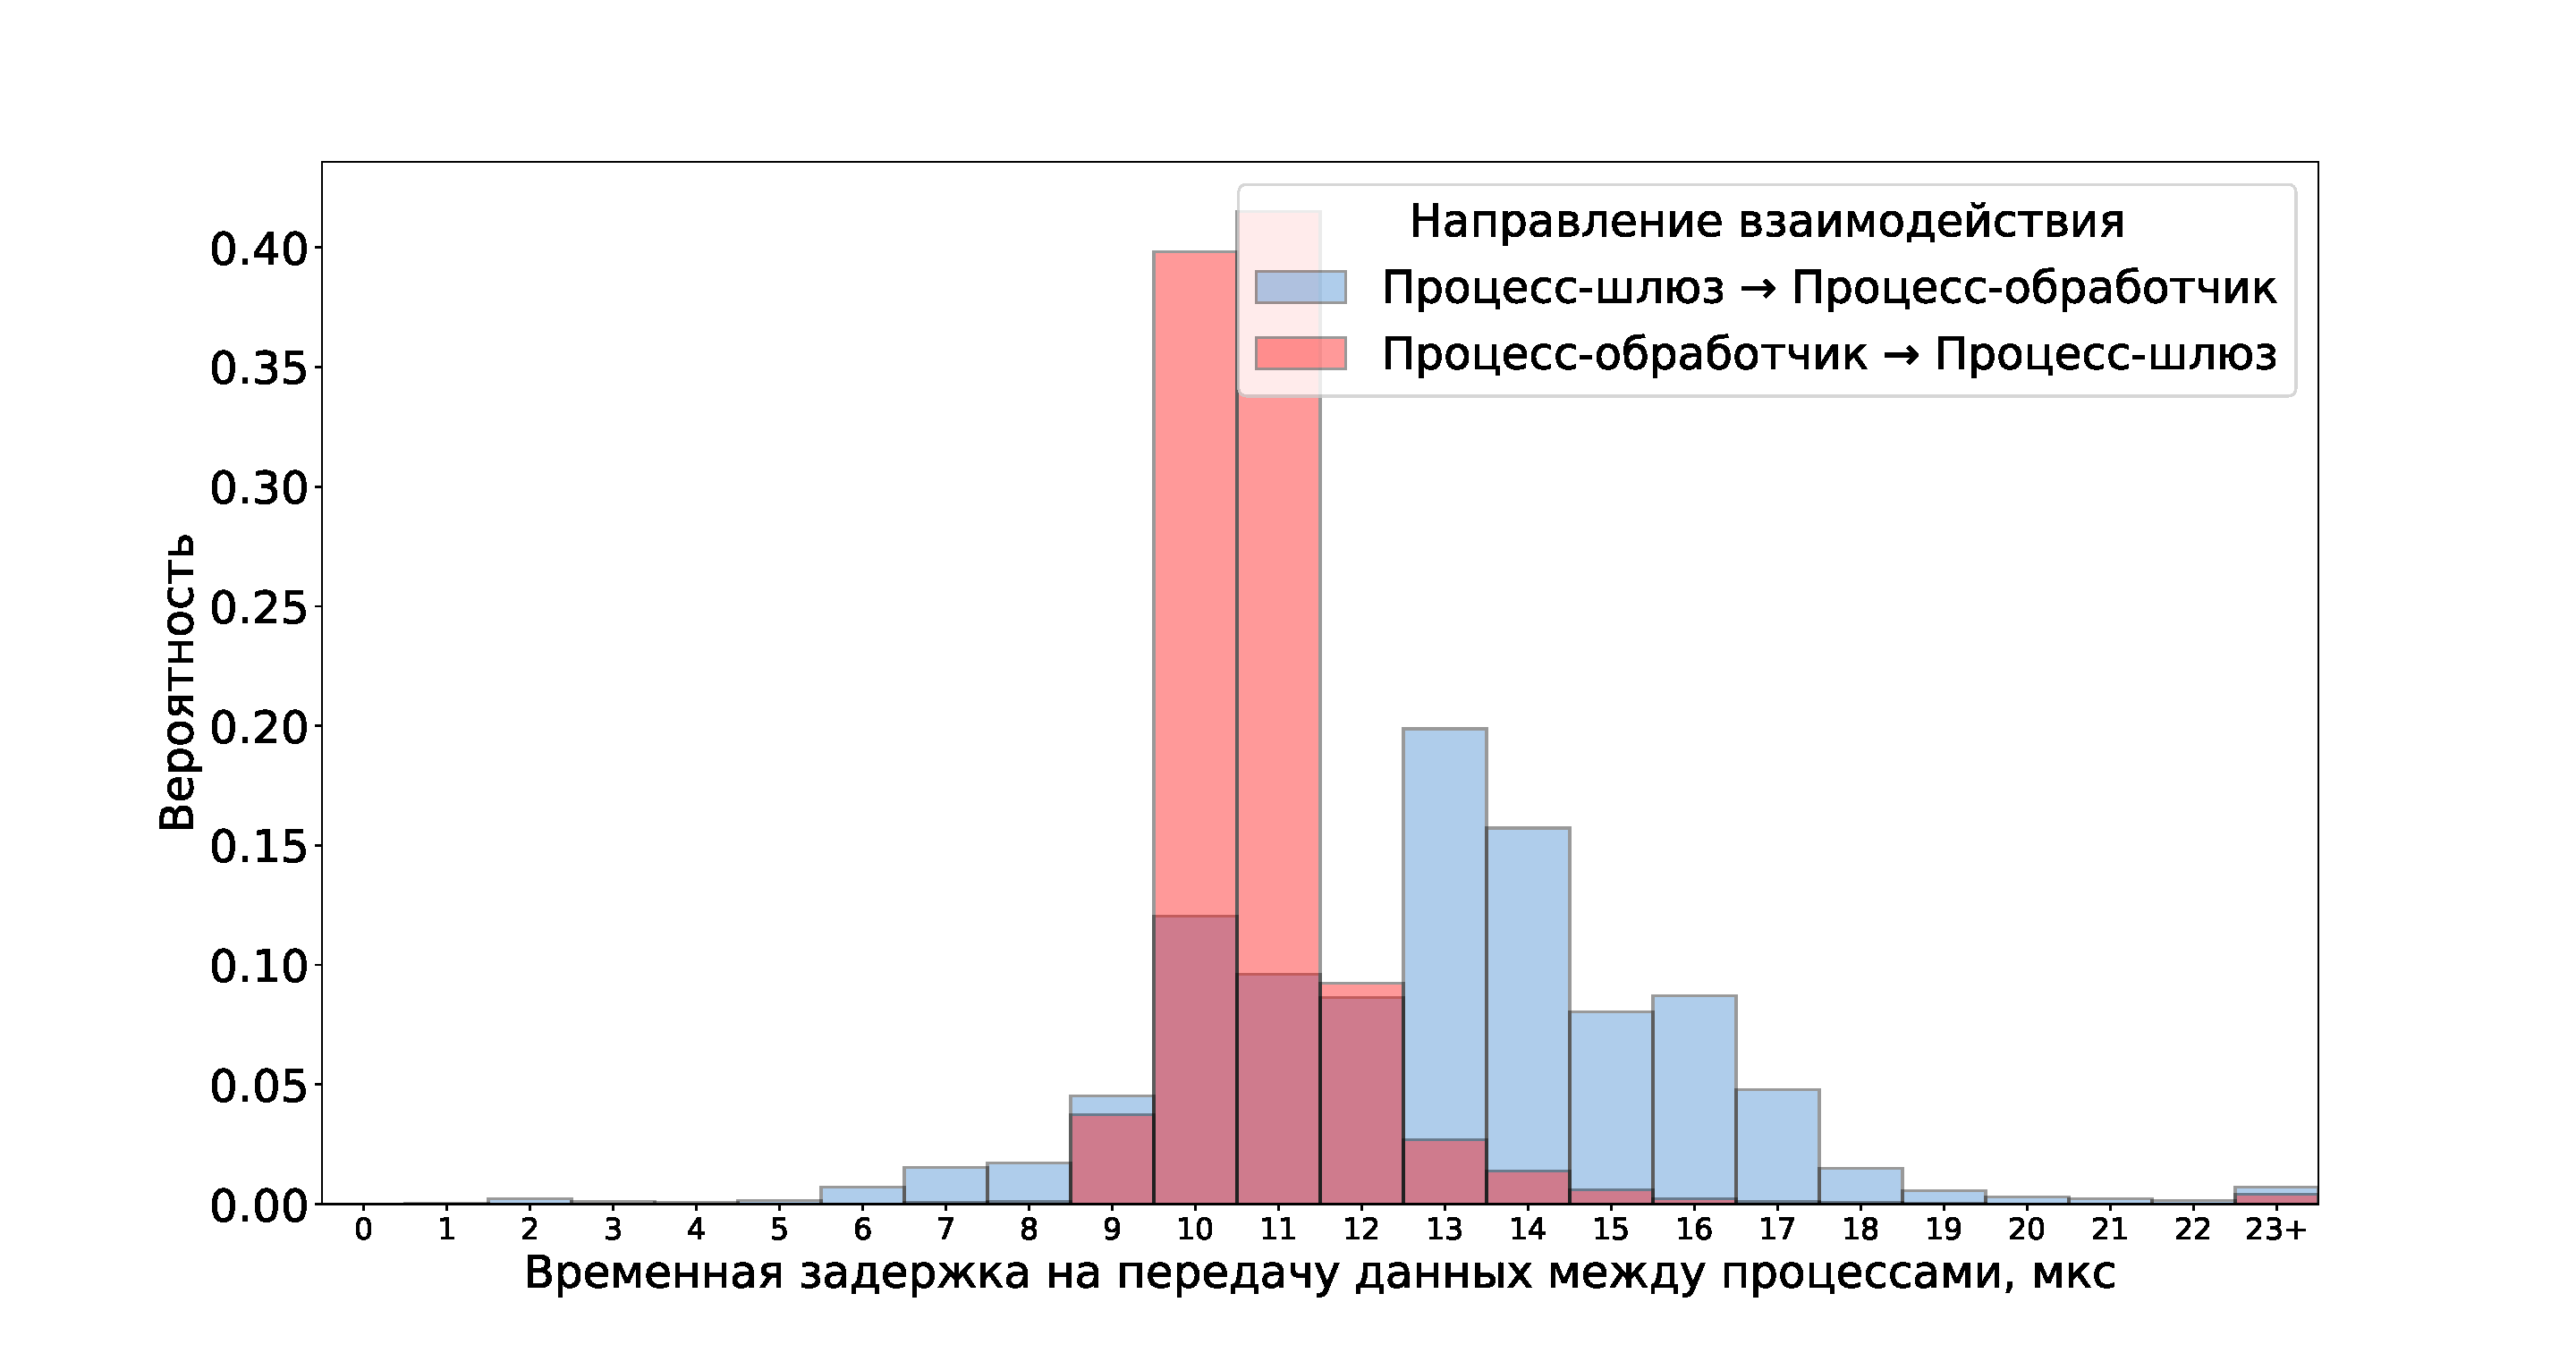
\includegraphics[width=\textwidth]{../../graphics/hist/BlockingHSHA}
\end{figure}

\begin{table}[!h]
\caption{Основные показатели временной задержки на передачу данных между процессами для метода, использующего разделяемую память для передачи данных, пассивное ожидание оповещений в мультиплексоре событий в разделяемой памяти и метод ''Полусинхронный/Полуреактивный`` при обслуживании заявок}\label{chapter41:TableBlockingHSHA}
\centering
\begin{tabular}{|l|c|c|}
\hline
\begin{tabular}[c]{@{}l@{}}Направление\\ взаимодействия/\\ Показатель\end{tabular} & \multicolumn{1}{l|}{\begin{tabular}[c]{@{}l@{}}Процесс-шлюз $\rightarrow$\\ Процесс-обработчик\end{tabular}} & \multicolumn{1}{l|}{\begin{tabular}[c]{@{}l@{}}Процесс-обработчик $\rightarrow$\\ Процесс-шлюз\end{tabular}} \\ \hline
min(t), мкс & 1 & 3 \\ \hline
M(t) $\pm$ 95\%, мкс & 12.5 $\pm$ 5.5 & 11.5 $\pm$ 2.5 \\ \hline
max(t), мс & 6.9 & 11.6 \\ \hline
\begin{tabular}[c]{@{}l@{}}$\Delta$, мс\end{tabular} & 10 $\pm$ 4 & 10 $\pm$ 4 \\ \hline
\begin{tabular}[c]{@{}l@{}}$\delta$, мкс\end{tabular} & 51 $\pm$ 28 & 92 $\pm$ 36 \\ \hline
\end{tabular}
\end{table}

В Таблице \ref{chapter41:TableBlockingHSHA} приведены основные временные характеристики данного метода. На Рисунке \ref{chapter41:FigBlockingHSHA} приведена гистограмма временной задержки на передачу данных для данного метода.

Использовании более эффективного метода межпроцессного взаимодействия наглядно показывает эффект от влияния времени обслуживания заявки в транспортном потоке на временную задержку на передачу данных. Процесс-шлюз с минимальной временной задержкой принимает и диспетчеризует заявку для дальнейшей обработки и сразу же готов принимать следующую заявку. Процесс-обработчик же использует транспортный поток для частичного обслуживания заявки (см. Рисунок \ref{chapter41:EngineLatency}), а потому в среднем временная задержка на передачу данных имеет худшие показатели, так как это может задерживать прием очередных заявок.

\paragraph{Диспетчеризация и обработка соединений по модели "Лидер/Последователи"}

Показатели потока исходящих заявок из симулятора в данном эксперименте: $\Delta \in$ \textit{10 $\pm$ 4 мс}, $\delta \in$ \textit{51 $\pm$ 28 мкс}.

В данном подразделе приведены данные об экспериментах с методом межпроцессного взаимодействия, описанным в Разделе \ref{chapter31:BlockingLF}.

В Таблице \ref{chapter41:TableBlockingLF} приведены основные временные характеристики данного метода.

На Рисунке \ref{chapter41:FigBlockingLF} приведена гистограмма временной задержки на передачу данных для данного метода.

\begin{figure}[!h]
\caption{Гистограмма временной задержки на передачу данных между процессами для метода, использующего разделяемую память для передачи данных, пассивное ожидание оповещений в мультиплексоре событий в разделяемой памяти и метод ''Лидер/Последователи`` при обслуживании заявок}
\label{chapter41:FigBlockingLF}
\includegraphics[width=\textwidth]{../../graphics/hist/BlockingLF}
\end{figure}

\begin{table}[!h]
\caption{Основные показатели временной задержки на передачу данных между процессами для метода, использующего разделяемую память для передачи данных, пассивное ожидание оповещений в мультиплексоре событий в разделяемой памяти и метод ''Лидер/Последователи`` при обслуживании заявок}\label{chapter41:TableBlockingLF}
\centering
\begin{tabular}{|l|c|c|}
\hline
\begin{tabular}[c]{@{}l@{}}Направление\\ взаимодействия/\\ Показатель\end{tabular} & \multicolumn{1}{l|}{\begin{tabular}[c]{@{}l@{}}Процесс-шлюз $\rightarrow$\\ Процесс-обработчик\end{tabular}} & \multicolumn{1}{l|}{\begin{tabular}[c]{@{}l@{}}Процесс-обработчик $\rightarrow$\\ Процесс-шлюз\end{tabular}} \\ \hline
min(t), мкс & 1 & 2 \\ \hline
M(t) $\pm$ 95\%, мкс & 11.5 $\pm$ 6.5 & 9.5 $\pm$ 1.5 \\ \hline
max(t), мс & 2.4 & 9.5 \\ \hline
\begin{tabular}[c]{@{}l@{}}$\Delta$, мс\end{tabular} & 10 $\pm$ 4 & 10 $\pm$ 4 \\ \hline
\begin{tabular}[c]{@{}l@{}}$\delta$, мкс\end{tabular} & 51 $\pm$ 28 & 89 $\pm$ 33 \\ \hline
\end{tabular}
\end{table}

По сравнению с методом ''Полусинхронный/Полуреактивный`` данный метод ожидаемо имеет меньшую временную задержку на передачу данных. В данном методе поток, получивший оповещение из мультиплексора событий, приступит к обработке сразу после того, как пробудит следующий поток-лидер. В то время как для предыдущего метода обработка заявки начнется только после пробуждения отдельного потока.
%Временная задержка на пробуждение другого потока ожидаемо ниже временной задержки на постановку этого потока на выполнение.

\paragraph{Выводы по исследованиям методов с пассивным ожиданием оповещений}

Методы оповещения процессов о появлении данных в разделяемой памяти с использованием мультиплексора в разделяемой памяти показывают существенно меньшую временную задержку на доставку оповещения, чем метод с использованием TCP. Это объясняется существенно меньшим количеством системных вызовов для обеих сторон взаимодействия.

Полученный результат подтверждает тезисы автора этих методов о превосходстве метода ''Лидер/Последователи`` над методом ''Полусинхронный/Полуреактивный`` при отсутствии необходимости приоритезации обработки заявок \cite[398]{schmidt2013pattern}. Однако, в отличие от исходного метода ''Полусинхронный/Полуреактивный`` \cite[375]{schmidt2013pattern}, работающего с сокетами и системным мультиплексором событий, в текущей ситуации нет необходимости считывать данные из сокета, чтобы переложить их в централизованную очередь для последующей обработки. Поэтому преимущество не такое существенное.

\subsubsection{Метод с активным ожиданием оповещений}

В методе с активным ожиданием оповещений поток мультиплексора событий находится в режиме постоянного опроса мультиплексора на предмет соединений (см. Раздел \ref{chapter31:NonBlockingLF}). В данном параграфе рассматривается исключительно метод обслуживания заявок ''Лидер/Последователи`` т.к. в параграфе выше он показал лучший результат по сравнению с методом обслуживания заявок ''Полусинхронный/Полуреактивный``.

\paragraph{Диспетчеризация и обработка соединений по модели "Лидер/Последователи"}

Показатели потока исходящих заявок из симулятора в данном эксперименте: $\Delta \in$ \textit{10 $\pm$ 4 мс}, $\delta \in$ \textit{51 $\pm$ 27 мкс}.

В данном подразделе приведены данные об экспериментах с методом межпроцессного взаимодействия, описанным в Разделе \ref{chapter31:NonBlockingLF}.

В Таблице \ref{chapter41:TableNonBlockingLF} приведены основные временные характеристики данного метода. На Рисунке \ref{chapter41:FigNonBlockingLF} приведена гистограмма временной задержки на передачу данных для данного метода.

\begin{figure}[!h]
\caption{Гистограмма временной задержки на передачу данных между процессами для метода, использующего разделяемую память для передачи данных, активно опрашиваемый мультиплексор в разделяемой памяти и модель ''Лидер/Последователи`` при обслуживании заявок}
\label{chapter41:FigNonBlockingLF}
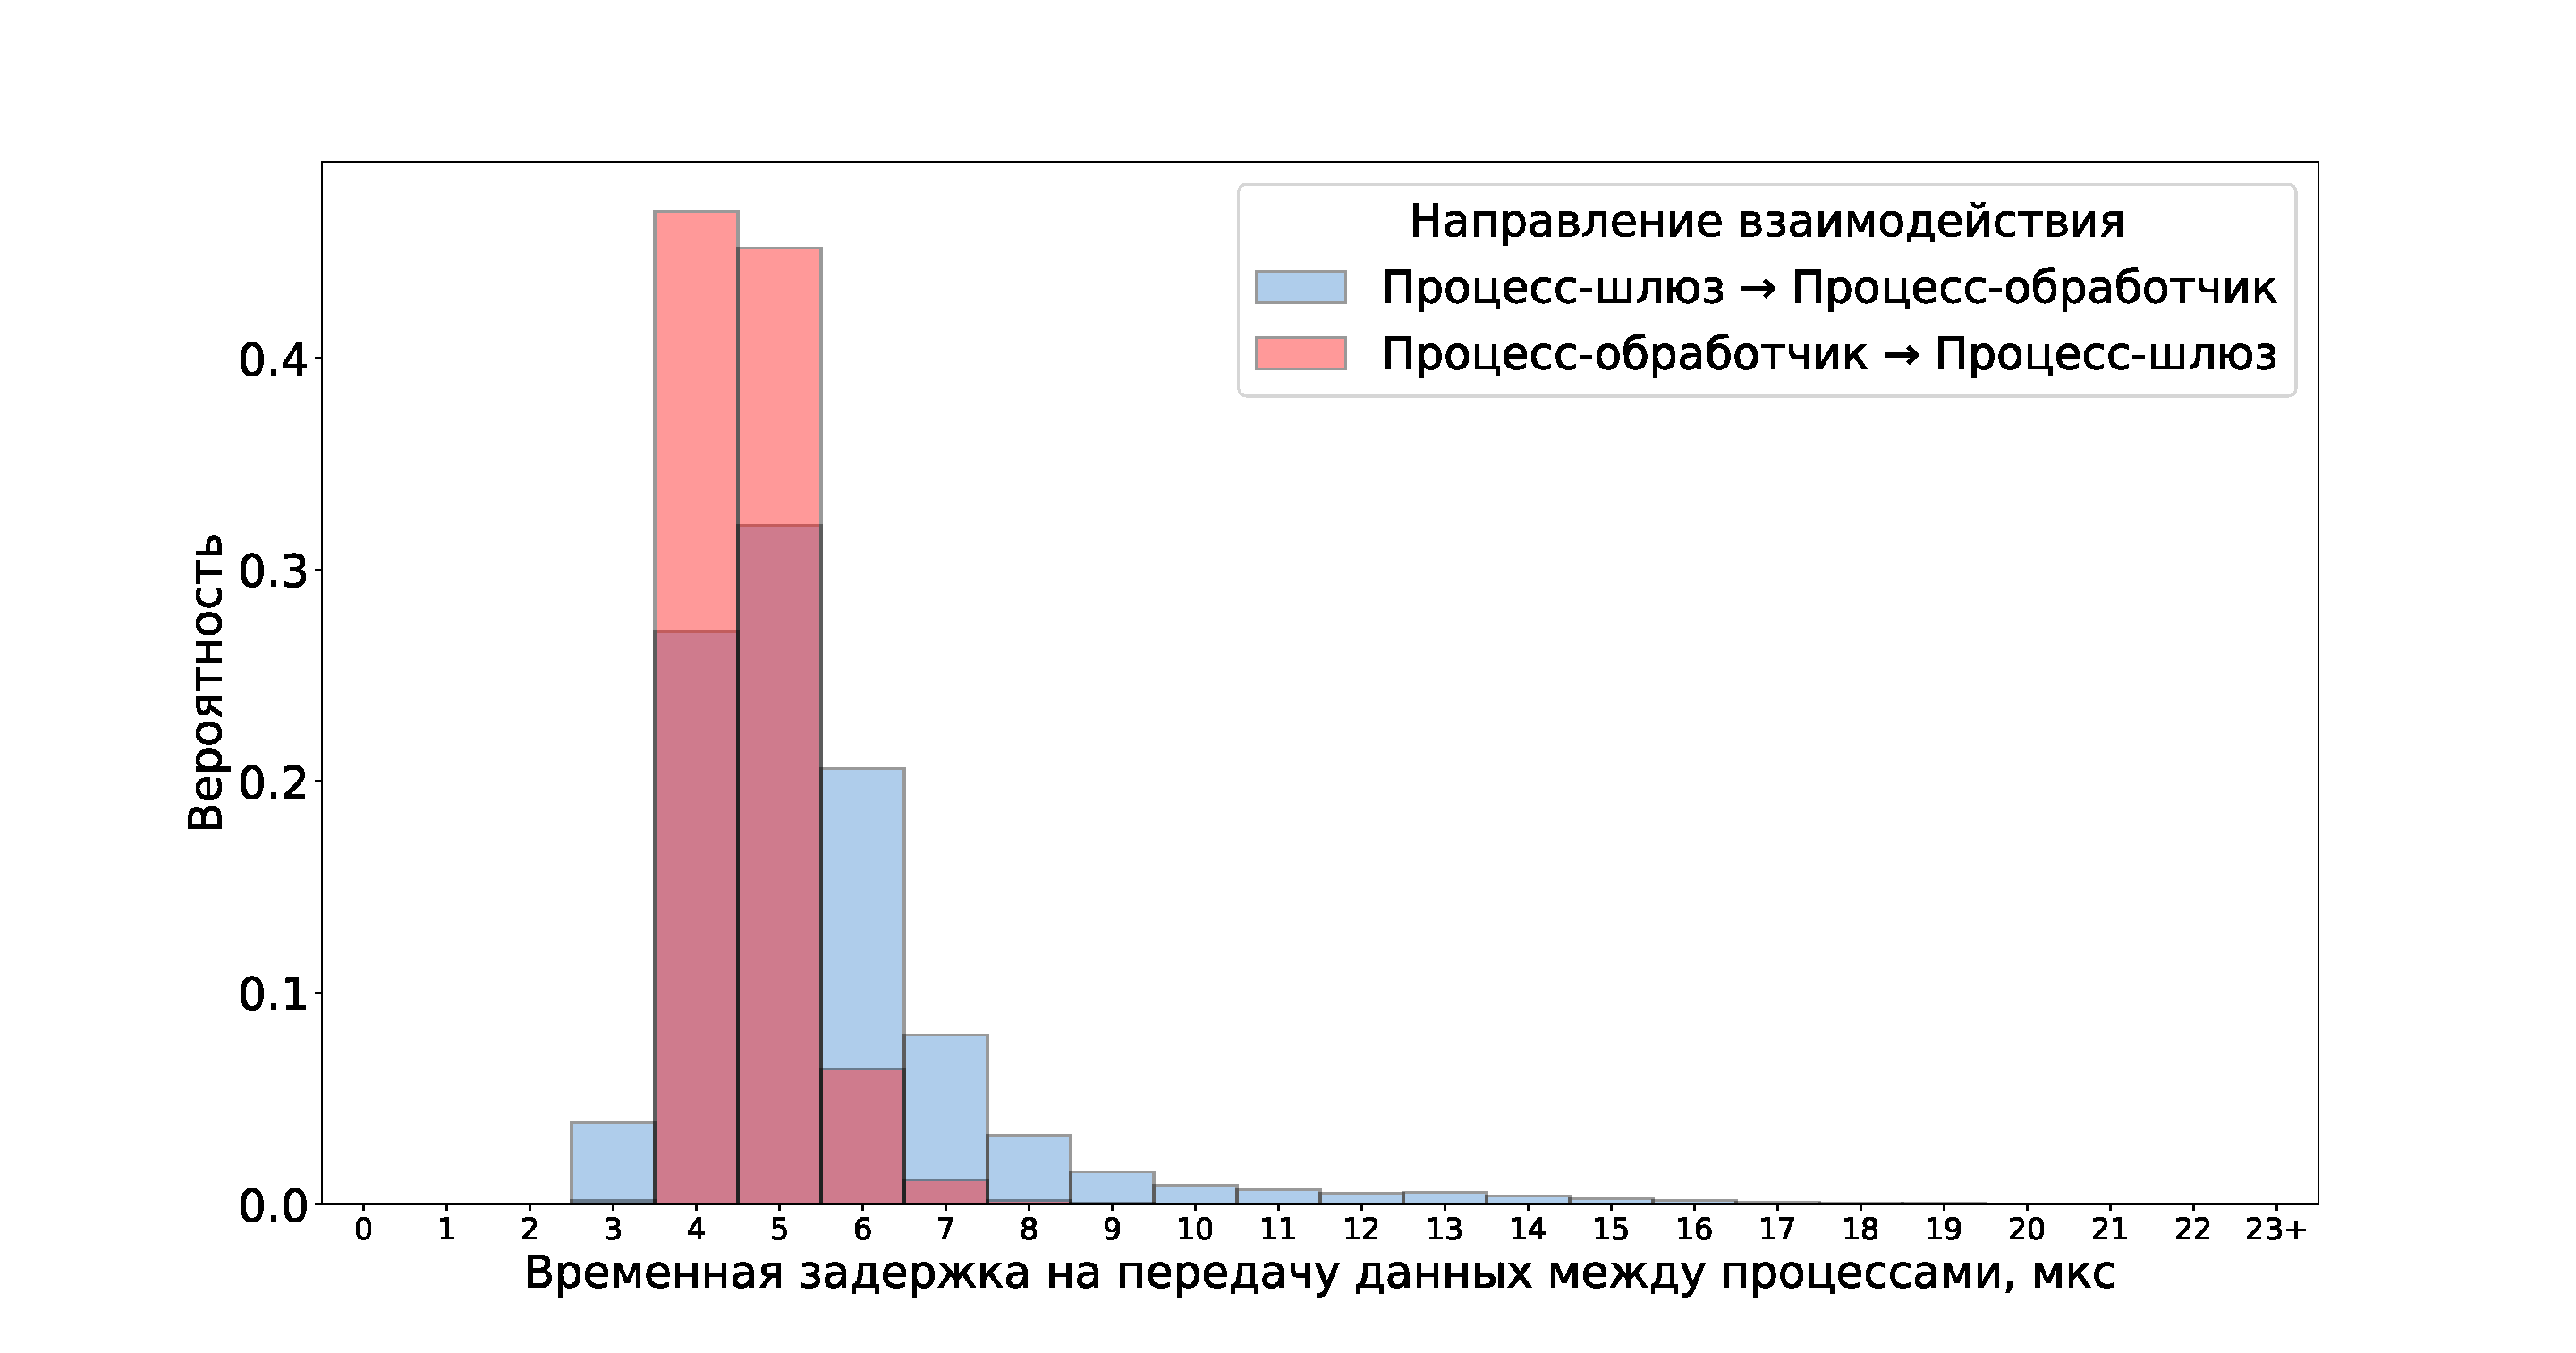
\includegraphics[width=\textwidth]{../../graphics/hist/NonBlockingLF}
\end{figure}

\begin{table}[!h]
\caption{Основные показатели временной задержки на передачу данных между процессами для метода, использующего разделяемую память для передачи данных, активно опрашиваемый мультиплексор в разделяемой памяти и модель ''Лидер/Последователи`` при обслуживании заявок}\label{chapter41:TableNonBlockingLF}
\centering
\begin{tabular}{|l|c|c|}
\hline
\begin{tabular}[c]{@{}l@{}}Направление\\ взаимодействия/\\ Показатель\end{tabular} & \multicolumn{1}{l|}{\begin{tabular}[c]{@{}l@{}}Процесс-шлюз $\rightarrow$\\ Процесс-обработчик\end{tabular}} & \multicolumn{1}{l|}{\begin{tabular}[c]{@{}l@{}}Процесс-обработчик $\rightarrow$\\ Процесс-шлюз\end{tabular}} \\ \hline
min(t), мкс & 1 & 3 \\ \hline
M(t) $\pm$ 95\%, мкс & 6 $\pm$ 2 & 5 $\pm$ 1 \\ \hline
max(t), мс & 0.064 & 0.017 \\ \hline
\begin{tabular}[c]{@{}l@{}}$\Delta$, мс\end{tabular} & 10 $\pm$ 4 & 10 $\pm$ 4 \\ \hline
\begin{tabular}[c]{@{}l@{}}$\delta$, мкс\end{tabular} & 51 $\pm$ 28 & 87 $\pm$ 33 \\ \hline
\end{tabular}
\end{table}

\paragraph{Выводы по исследованию метода с активным ожиданием}
Метод с активным ожиданием событий в мультиплексоре в разделяемой памяти ожидаемо показывает лучший результат по сравнению со всеми ранее рассмотренными методами. Это происходит потому что в данном случае нет необходимости пробуждать и дожидаться пробуждения потока для обслуживания заявки. Исходя из разницы временной задержки на передачу данных в методах с активным и пассивным ожиданием, пробуждение потока до постановки его на выполнение занимает около 5-6 мкс.
% \textbf{TBD: а надо ли оно мне? Вопрос корректности приведения циклов на AMD к секундам спорный}
В работе другого автора \cite{8526899} была измерена временная задержка на пробуждение потоков, прикрепленных к разным ядрам разных процессоров, посредством системного вызова futex. Измерения проводились на процессоре AMD Opteron 6272 и показали $\mu = 24640.5$ машинных циклов от системного вызова до выполнения первой инструкции пробужденным потоком. Или $\frac{24640.5~\text{машинных~циклов}}{2.1~*~10^9~\text{Гц}} \approx 11 ~\text{мкс}$ при частоте процессора 2.1 ГГц, что похоже на обозначенный выше результат с учетом использования в настоящей работе более современного аппаратного обеспечения.

Для данного метода распределение временной задержки на передачу данных от процесса-обработчика к процессу-шлюзу схоже с предыдущими методами, но этот показатель существенно отличается при передаче от процесса-шлюза к процессу-обработчику. Это может быть вызвано тем, что более быстрый метод межпроцессного взаимодействия при данной постановке эксперимента приводит к отсутствию и, как следствие, время обслуживания заявки в транспортном потоке процесса-обработчика не влияет на временную задержку на передачу данных.

Данный подход обладает существенным \textbf{недостатком}. Поскольку поток, активно опрашивающий мультиплексор, исполняется до получения и обработки события, то существует возможность, что планировщик ОС вытеснит этот поток с процессора. Стандартный квант планирования потоков в Linux -- 100 мс. Если событие не будет получено и обработано за это время, то поток может быть вытеснен с процессора и временная задержка на передачу данных увеличится на сотни миллисекунд. Данный недостаток не проявляется в проведенном эксперименте, поскольку что интервал $\Delta$ между сериями заявок значительно меньше 100 мс.
